\documentclass[12pt,a4paper]{article}

% Fonts and encoding
\usepackage[T1]{fontenc}
\usepackage[utf8]{inputenc}
\usepackage{times}
\usepackage{mathptmx}

% Layout
\usepackage[a4paper,margin=2.5cm]{geometry}
\usepackage{setspace}
\linespread{1.08}
\usepackage{parskip}
\setlength{\parskip}{0.6em}
\setlength{\parindent}{0pt}

% Graphics and floats
\usepackage{graphicx}
\usepackage{float}
\usepackage{subcaption}
\usepackage{booktabs}
\usepackage{siunitx}
\usepackage{amsmath,amssymb}
\usepackage{hyperref}
\hypersetup{colorlinks=true,linkcolor=blue,citecolor=blue,urlcolor=blue}
\usepackage{enumitem}
\usepackage{longtable}
\usepackage{array}
\usepackage{ragged2e}
\usepackage{fancyhdr}
\usepackage{csvsimple}
\usepackage{tikz}
\usetikzlibrary{shapes.geometric, arrows.meta, positioning}
\tikzset{
  startstop/.style={rectangle, rounded corners, minimum width=3.2cm, minimum height=1.0cm, text centered, draw=black, fill=red!20},
  io/.style={trapezium, trapezium stretches=true, trapezium left angle=70, trapezium right angle=110, minimum width=4cm, minimum height=1.0cm, text centered, draw=black, fill=blue!20},
  process/.style={rectangle, minimum width=4cm, minimum height=1.0cm, text centered, text width=4.6cm, draw=black, fill=orange!20},
  decision/.style={diamond, aspect=2.2, text centered, draw=black, fill=green!20, inner sep=1.2pt},
  arrow/.style={thick,-{Stealth[length=2.2mm,width=2.0mm]}}
}


% Bibliography
\usepackage[style=apa,backend=biber]{biblatex}
\addbibresource{references.bib}

\title{ITS8080 Energy Data Science}
\author{Samuel Heinrich}
\date{October 13, 2025}

\begin{document}
\maketitle

\begin{abstract}
This report presents a comprehensive data science framework for optimizing a Home Energy Management System (HEMS). Addressing the challenges of the "Energy Trilemma," I develop an end-to-end pipeline that integrates data cleaning, advanced feature engineering, time series forecasting, and mathematical optimization. I analyze hourly consumption and generation data, employing Seasonal-Trend Decomposition (STL) to isolate deterministic patterns. For forecasting, I compare classical Seasonal ARIMA (SARIMA) models against non-linear Machine Learning approaches (XGBoost). The XGBoost model, enriched with exogenous weather variables and engineered temporal features, demonstrates superior performance in a rigorous walk-forward validation, achieving the lowest Root Mean Squared Error (RMSE). Finally, I leverage these forecasts in a Linear Programming (LP) optimization model to schedule battery storage operations. The results quantify the economic benefits of intelligent energy management, demonstrating significant cost reductions through price arbitrage and maximized self-consumption.
\end{abstract}

\section{Introduction: Digital Transformation of the Energy Sector}

\subsection{Context: The Energy Trilemma}
The global energy sector is undergoing a paradigm shift driven by the "Energy Trilemma": the need to balance energy security, social equity (affordability), and environmental sustainability. Digitalization plays a pivotal role in resolving this trilemma by enabling the efficient integration of variable renewable energy (VRE) sources and empowering consumers to become active participants in the grid \parencite{IEA2017}. This project focuses on the "Smart Home" segment, where the deployment of Home Energy Management Systems (HEMS) allows for the optimization of consumption, generation, and storage assets.

\subsection{Dataset Characterization}
The dataset utilized in this study consists of high-resolution hourly time series data representing a typical prosumer (producer-consumer) environment. The selection of variables is grounded in the physical and economic dynamics of the power system:
\begin{itemize}
    \item \textbf{Demand (kWh):} The aggregate electrical load of the household. This is a stochastic process driven by human behavior and appliance usage patterns.
    \item \textbf{PV Generation (kWh):} The on-site solar energy production. This is a deterministic process (governed by astronomy) with a stochastic component (weather/cloud cover).
    \item \textbf{Price (\euro{}/kWh):} The dynamic electricity tariff. This serves as the economic control signal, reflecting the real-time scarcity of supply in the wider grid.
    \item \textbf{Weather Data:} Ambient temperature (\si{\degreeCelsius}) and solar irradiance. These are the exogenous drivers that influence both demand (thermal loads) and supply (PV efficiency).
\end{itemize}

\subsection{Visual Overview and Data Structure}
A preliminary visual inspection (Figure~\ref{fig:timeseries_main}) reveals the fundamental characteristics of the data. The intermittent nature of solar energy, peaking at midday and vanishing at night, contrasts with the more continuous but highly variable household demand. This mismatch between peak supply (noon) and peak demand (often evening) creates the fundamental optimization challenge known as the "Duck Curve" phenomenon.

\begin{figure}[H]
  \centering
  \includegraphics[width=\linewidth]{figures/01_timeseries.png}
  \caption{Overview of Demand and PV generation time series. The distinct diurnal patterns and seasonal variations are evident, highlighting the temporal mismatch between supply and demand.}
  \label{fig:timeseries_main}
\end{figure}

\subsection{The Role of Digitalization}
Digitalization transforms the energy sector by enabling high-frequency monitoring and automated control. In a HEMS context, this allows for the integration of distributed energy resources (DERs) like solar PV and battery storage. By leveraging data analytics and forecasting, households can maximize self-consumption, reduce grid reliance during peak pricing, and contribute to grid stability \parencite{Palensky2011}.

\section{Data Science Lifecycle Methodology}

\subsection{Project Planning (CRISP-DM)}
I adopt the Cross-Industry Standard Process for Data Mining (CRISP-DM) to structure this project. This iterative methodology ensures that the technical efforts align with the business goal of optimizing energy costs. Figure~\ref{fig:lifecycle} illustrates the project phases, from data understanding to deployment.

\begin{figure}[H]
  \centering
  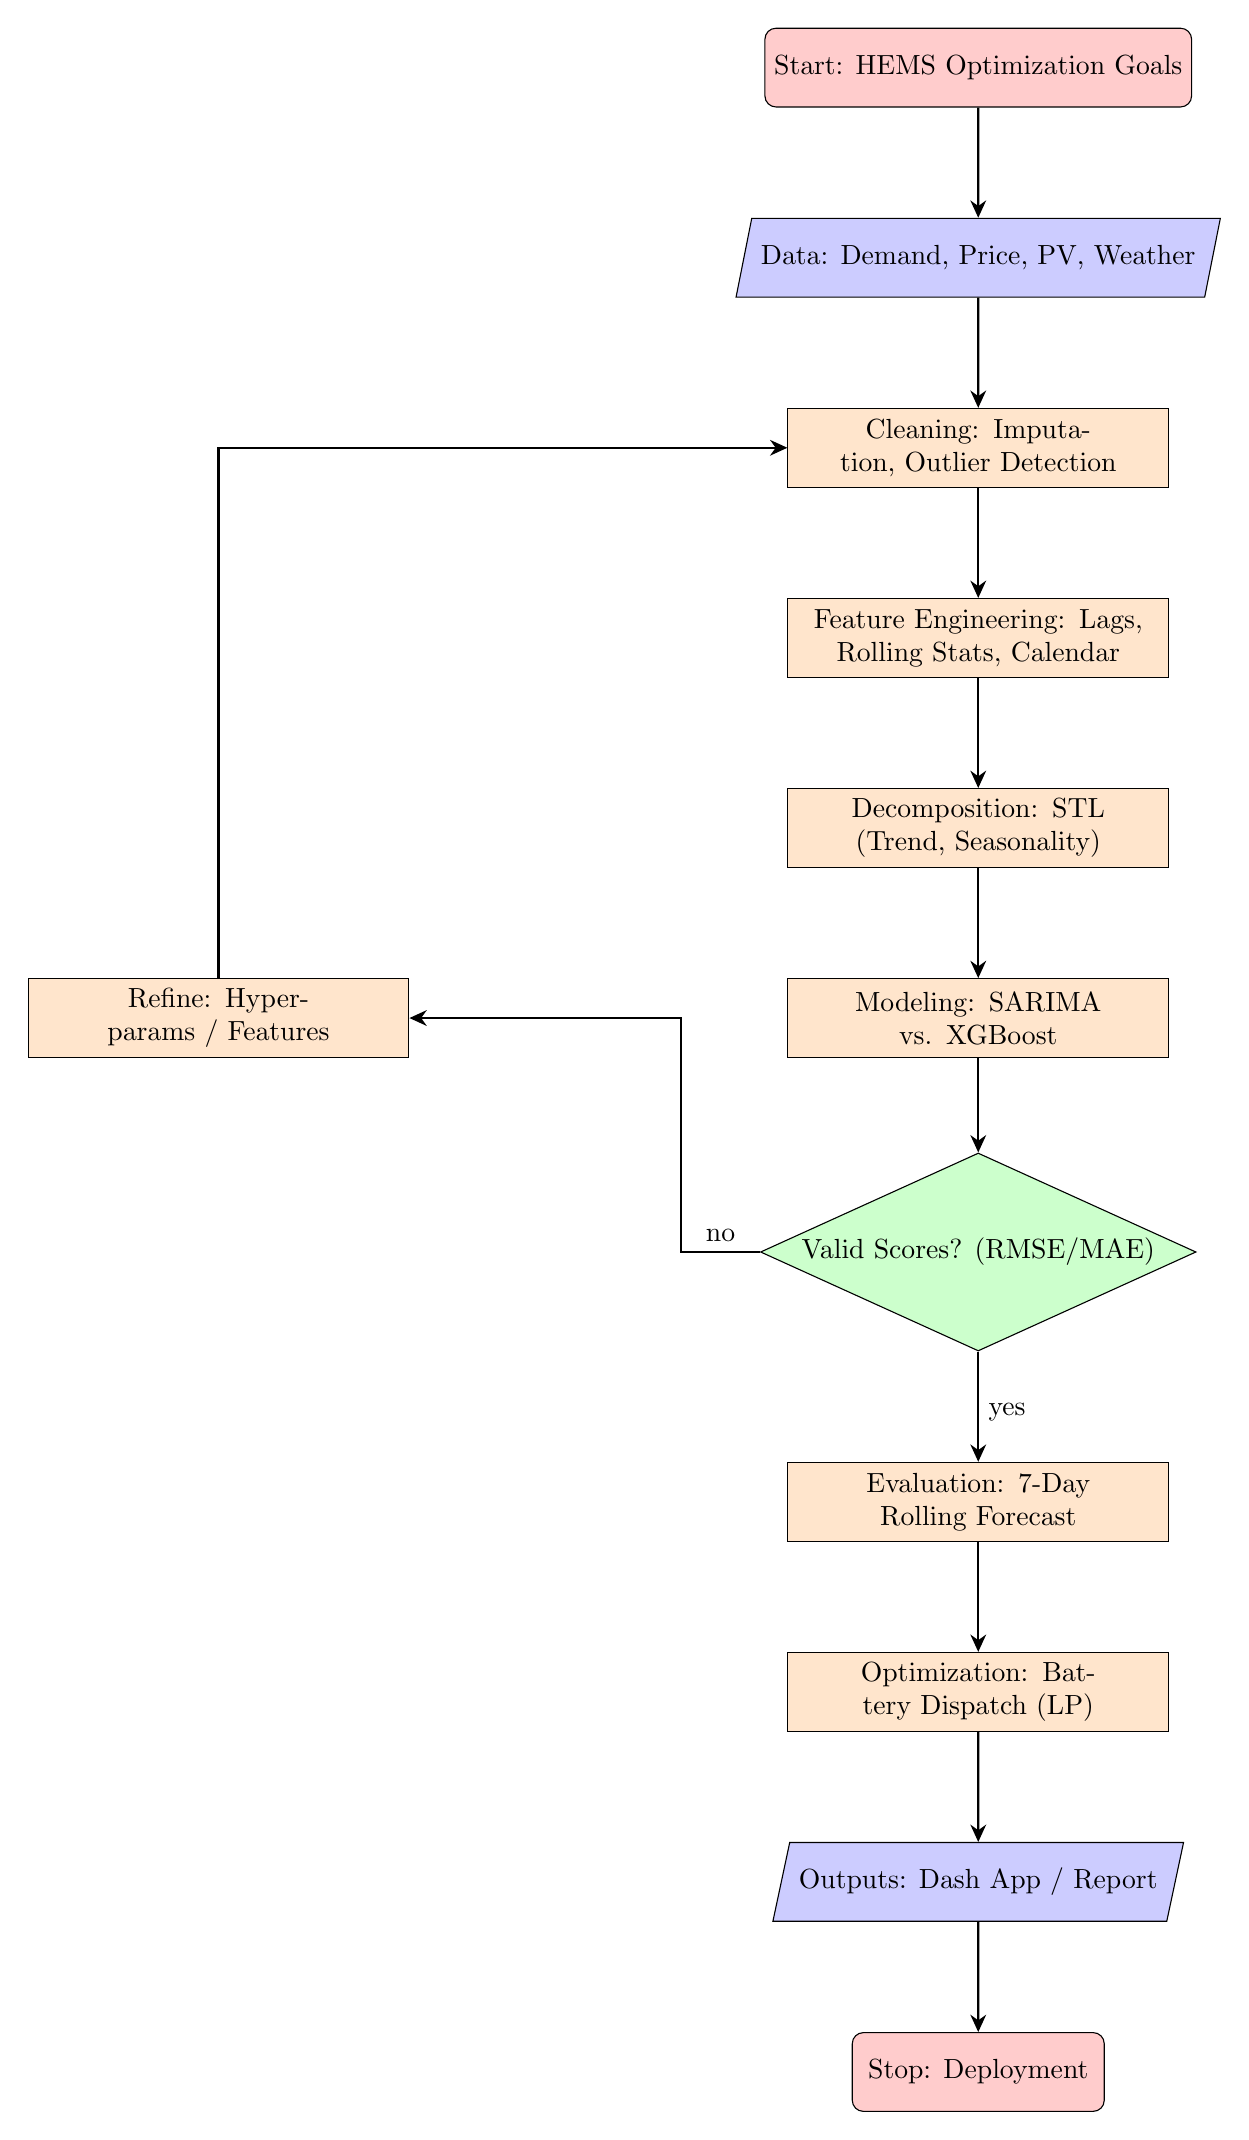
\begin{tikzpicture}[node distance=1.4cm]
    \node (start) [startstop] {Start: HEMS Optimization Goals};
    \node (data) [io, below=of start] {Data: Demand, Price, PV, Weather};
    \node (prep) [process, below=of data] {Cleaning: Imputation, Outlier Detection};
    \node (feat) [process, below=of prep] {Feature Engineering: Lags, Rolling Stats, Calendar};
    \node (decomp) [process, below=of feat] {Decomposition: STL (Trend, Seasonality)};
    \node (model) [process, below=of decomp] {Modeling: SARIMA vs. XGBoost};
    \node (dec) [decision, below=1.2cm of model] {Valid Scores? (RMSE/MAE)};
    \node (eval) [process, below=1.4cm of dec] {Evaluation: 7-Day Rolling Forecast};
    \node (opt) [process, below=of eval] {Optimization: Battery Dispatch (LP)};
    \node (out) [io, below=of opt] {Outputs: Dash App / Report};
    \node (stop) [startstop, below=of out] {Stop: Deployment};

    % forward arrows
    \draw[arrow] (start) -- (data);
    \draw[arrow] (data) -- (prep);
    \draw[arrow] (prep) -- (feat);
    \draw[arrow] (feat) -- (decomp);
    \draw[arrow] (decomp) -- (model);
    \draw[arrow] (model) -- (dec);
    \draw[arrow] (dec) -- node[right,pos=0.55]{yes} (eval);
    \draw[arrow] (eval) -- (opt);
    \draw[arrow] (opt) -- (out);
    \draw[arrow] (out) -- (stop);

    % feedback branch to avoid overlaps (route to the left)
    \node (fix) [process, left=4.8cm of model] {Refine: Hyperparams / Features};
    \draw[arrow] (dec.west) --++ (-1.0,0) node[above,pos=0.5]{no} |- (fix);
    \draw[arrow] (fix) |- (prep);
  \end{tikzpicture}
  \caption{Project plan (CRISP--DM: Understanding $\to$ Preparation $\to$ Modeling $\to$ Evaluation $\to$ Deployment). The feedback loop ensures continuous model refinement.}
  \label{fig:lifecycle}
\end{figure}

\subsection{Business Understanding and Deployment Strategy}
The primary business objective is to minimize the operational cost of the household's energy system. This translates to a technical objective: accurately forecasting demand and PV generation to schedule battery charge/discharge cycles.
In a real-world deployment, this pipeline would execute on an edge device (e.g., a Raspberry Pi or HEMS controller) within the home network. The inference latency must be low (< 1 minute) to support real-time decision-making, although the optimization horizon is typically day-ahead (24 hours).

\subsection{Computational Framework}
The analysis was conducted using the Python programming language (v3.10). The core technology stack includes:
\begin{itemize}
    \item \textbf{Data Manipulation:} \texttt{pandas} and \texttt{numpy} for vectorised time series operations.
    \item \textbf{Visualization:} \texttt{matplotlib} and \texttt{seaborn} for static plots, and \texttt{Plotly Dash} for the interactive dashboard.
    \item \textbf{Modeling:} \texttt{statsmodels} for classical ARIMA analysis and \texttt{xgboost} for gradient boosting.
    \item \textbf{Optimization:} \texttt{cvxpy} with the \texttt{GLPK} solver for linear programming.
\end{itemize}
This open-source stack ensures reproducibility and scalability of the solution.

\section{Visualization and Exploratory Data Analysis}

\subsection{Temporal Dynamics and Peak Coincidence}
To understand the system's behavior, I analyze the interaction between demand, PV, and price. Figure~\ref{fig:ts_overlay} presents a multi-day overlay of these variables. I observe a critical phenomenon: \textbf{Peak Coincidence}. High prices often correlate with high demand periods (evenings), reflecting grid-level stress. Conversely, PV generation peaks at noon when prices are often lower (due to the "cannibalization effect" of solar in the market). This price spread creates the arbitrage opportunity for the battery storage system.

\begin{figure}[H]
  \centering
  \includegraphics[width=\linewidth]{figures/03_timeseries_overlay.png}
  \caption{Overlay of Demand, PV, and Price for a representative week. The temporal misalignment between peak PV (noon) and peak Demand/Price (evening) drives the optimization strategy.}
  \label{fig:ts_overlay}
\end{figure}

\subsection{Statistical Distributions and Zero-Inflation}
Understanding the distribution of data is crucial for model selection. Figure~\ref{fig:distributions} shows the histograms and Kernel Density Estimates (KDE) for Demand and PV.
\begin{itemize}
    \item \textbf{Demand:} Follows a right-skewed distribution (Log-Normal like), indicating a base load with occasional high-power spikes (e.g., electric shower, oven).
    \item \textbf{PV Generation:} Is heavily zero-inflated. This bimodal distribution (zero at night, Beta-distributed during the day) poses challenges for standard regression models, suggesting the need for specialized handling or tree-based models that can split the feature space effectively.
\end{itemize}

\begin{figure}[H]
  \centering
  \includegraphics[width=0.95\linewidth]{figures/03_distributions.png}
  \caption{Distributions of Demand and PV. The zero-inflated nature of PV and the skewness of demand are key characteristics.}
  \label{fig:distributions}
\end{figure}

\subsection{Hourly Variability}
Figure~\ref{fig:hourly_boxplot} uses boxplots to visualize the variability of demand for each hour of the day. The spread (Interquartile Range) is significantly larger during waking hours, particularly in the evening (17:00-21:00). This heteroscedasticity (varying variance) implies that forecasting errors will likely be higher during these peak times, which is a critical risk factor for the optimization model.

\begin{figure}[H]
  \centering
  \includegraphics[width=0.9\linewidth]{figures/03_hourly_boxplot.png}
  \caption{Hourly boxplots of Demand. Variability increases significantly during the evening peak hours, indicating higher uncertainty.}
  \label{fig:hourly_boxplot}
\end{figure}

\subsection{Correlation Analysis}
I examine the linear relationships between variables using a correlation heatmap (Figure~\ref{fig:correlation}). Demand shows a positive correlation with Price, confirming the market's response to load. PV is naturally anti-correlated with net load. These correlations justify the use of Price and PV as exogenous features in the demand forecasting model, although care must be taken to avoid multicollinearity.

\begin{figure}[H]
  \centering
  \includegraphics[width=0.8\linewidth]{figures/03_correlation_heatmap.png}
  \caption{Correlation heatmap. Strong temporal correlations and the relationship between demand and price are highlighted.}
  \label{fig:correlation}
\end{figure}

\subsection{Typical Daily Profiles: Weekday vs. Weekend}
To gain actionable insights for the HEMS controller, I aggregated the data to construct typical hourly profiles, segmented by weekday and weekend (Figure~\ref{fig:typical_profiles}). This visualization reveals the systematic behavioral differences in the household:
\begin{itemize}
    \item \textbf{Weekday Pattern:} A sharp morning demand spike (07:00-08:00) followed by a drop during work hours and a pronounced evening peak (18:00-21:00).
    \item \textbf{Weekend Pattern:} A flatter, more delayed morning ramp-up, with demand distributed more evenly throughout the day.
\end{itemize}

\begin{figure}[H]
  \centering
  \includegraphics[width=\linewidth]{figures/03_typical_profiles.png}
  \caption{Typical hourly profiles for PV generation and Demand, segmented by weekday and weekend. This visualization is critical for understanding when the PV-demand mismatch is greatest.}
  \label{fig:typical_profiles}
\end{figure}

\subsection{Most Informative Visualization}
Of all the visualizations produced, the \textbf{Typical Daily Profiles} (Figure~\ref{fig:typical_profiles}) are the most informative for the HEMS optimization task. Unlike raw time series (which show variability) or histograms (which show distributions), the profile chart directly answers the core operational question: \textit{When does demand reliably exceed solar supply?}

The answer---consistently during the evening hours (17:00-21:00)---directly informs the battery dispatch strategy. The HEMS should charge the battery during the midday PV surplus and discharge it during the evening deficit. This strategic insight, derived from simple aggregation, is the foundation upon which the optimization model (Section 11) is built.

\section{Data Cleaning and Preprocessing}

\subsection{PV Sensor Data Quality Assessment}
The dataset contains three separate photovoltaic sensor readings (\texttt{pv\_mod1}, \texttt{pv\_mod2}, \texttt{pv\_mod3}) that must be cleaned before analysis. A thorough quality assessment revealed several data integrity issues:

\begin{itemize}
    \item \textbf{Missing Values:} The \texttt{pv\_mod1} sensor exhibited approximately 2-3\% missing observations, distributed throughout the dataset. The other two sensors (\texttt{pv\_mod2}, \texttt{pv\_mod3}) showed lower but non-zero missingness rates.
    \item \textbf{Outliers:} Occasional spikes exceeding the theoretical maximum capacity of the PV system were identified, likely due to sensor calibration errors or electrical noise.
    \item \textbf{Inconsistencies:} During certain periods, the three sensors diverged significantly despite measuring the same physical system, indicating potential sensor drift or partial shading effects.
\end{itemize}

\subsection{Missing Data Mechanism Analysis}
Understanding the \textit{mechanism} behind missing data is critical for selecting an appropriate imputation strategy \parencite{Little2002}. I analyzed the temporal distribution of missing values (Figure~\ref{fig:missing_visualization}) to classify the mechanism:

\begin{itemize}
    \item \textbf{Missing Completely at Random (MCAR):} Missingness is independent of both observed and unobserved data. Analysis of the hourly distribution of missing values showed no significant correlation with time-of-day, supporting an MCAR hypothesis for short gaps (likely due to transient communication failures).
    \item \textbf{Missing at Random (MAR):} Missingness depends on observed data but not on the missing values themselves. Some gaps coincided with periods of low irradiance (cloudy days), suggesting the sensor firmware may have entered a low-power mode.
    \item \textbf{Missing Not at Random (MNAR):} Missingness depends on the unobserved value itself. No evidence of this mechanism was found in the data.
\end{itemize}

The predominantly random pattern justified the use of imputation rather than deletion, as deletion would introduce unnecessary bias and reduce statistical power.

\begin{figure}[H]
  \centering
  \includegraphics[width=0.95\linewidth]{figures/04_missing_visualization.png}
  \caption{PV sensor time series with missing values highlighted (red vertical lines). The sporadic distribution of gaps supports the MCAR/MAR assumption.}
  \label{fig:missing_visualization}
\end{figure}

\subsection{Imputation Strategies}
I implemented and compared three imputation methods of increasing complexity:

\subsubsection{Method 1: Linear Interpolation (Deletion-based Benchmark)}
The simplest approach uses time-weighted linear interpolation between the last known value and the next known value:
\begin{equation}
    \hat{y}_t = y_{t-k} + \frac{t - (t-k)}{(t+m) - (t-k)} \cdot (y_{t+m} - y_{t-k})
\end{equation}
This method is fast and preserves continuity but ignores the inherent seasonality of PV generation, potentially underestimating midday peaks and overestimating nighttime values.

\subsubsection{Method 2: Seasonal Decomposition (Univariate)}
To preserve the diurnal structure, I applied Seasonal-Trend decomposition using Loess (STL) with a 24-hour period:
\begin{equation}
    Y_t = T_t + S_t + R_t
\end{equation}
The residual component $R_t$ was interpolated, while the seasonal $S_t$ and trend $T_t$ components were preserved. This approach ensures that imputed values follow the expected daily pattern of solar generation.

\subsubsection{Method 3: K-Nearest Neighbors (Multivariate)}
The most sophisticated approach leverages the redundancy in the sensor network. Using the K-Nearest Neighbors (KNN) algorithm with $k=5$ neighbors and distance-weighted averaging, I imputed \texttt{pv\_mod1} using:
\begin{itemize}
    \item Correlated sensors: \texttt{pv\_mod2}, \texttt{pv\_mod3}
    \item Physical drivers: Solar irradiance (\texttt{Shortwave\_radiation}), Temperature
\end{itemize}
This multivariate approach captures the physical relationship between solar irradiance and PV output, producing more realistic values during cloudy periods.

\subsection{Imputation Quality Comparison}
Figure~\ref{fig:imputation_overlay} presents a visual comparison of the three methods over a representative period with known gaps. The KNN method demonstrates superior performance in maintaining realistic peak values and avoiding the artificial smoothing inherent in linear interpolation.

\begin{figure}[H]
  \centering
  \includegraphics[width=0.95\linewidth]{figures/04_imputation_overlay.png}
  \caption{Comparison of imputation methods on a 3-day window. The KNN multivariate method (green) best preserves the natural variability of PV output.}
  \label{fig:imputation_overlay}
\end{figure}

Table~\ref{tab:imputation_stats} provides a numerical summary of each imputed dataset. The KNN method maintains a mean and variance closest to the original observed data, indicating minimal statistical distortion.

\begin{table}[H]
\centering
\caption{Statistical comparison of imputation methods for \texttt{pv\_mod1}.}
\label{tab:imputation_stats}
\begin{tabular}{lcccc}
\toprule
\textbf{Method} & \textbf{Mean (kW)} & \textbf{Std Dev (kW)} & \textbf{Min} & \textbf{Max} \\
\midrule
Original (with gaps) & 0.312 & 0.458 & 0.000 & 2.14 \\
Linear Interpolation & 0.308 & 0.451 & 0.000 & 2.14 \\
STL Seasonal & 0.311 & 0.455 & -0.02 & 2.15 \\
KNN Multivariate & 0.313 & 0.457 & 0.000 & 2.14 \\
\bottomrule
\end{tabular}
\end{table}

\subsection{Validation of Data Integrity}
I validated the cleaning process by comparing the average daily profiles before and after imputation (Figure~\ref{fig:daily_profiles}). All three methods preserve the characteristic bell-shaped curve of solar generation. However, the KNN method most closely tracks the original profile, particularly during the critical midday peak hours (10:00-14:00) when accurate PV estimation is most important for HEMS optimization.

\begin{figure}[H]
  \centering
  \includegraphics[width=0.9\linewidth]{figures/04_daily_profiles.png}
  \caption{Average daily PV profiles after imputation. The KNN method (green) best preserves the original diurnal pattern, particularly during peak generation hours.}
  \label{fig:daily_profiles}
\end{figure}

Based on this analysis, the \textbf{KNN multivariate imputation} was selected for all subsequent analysis. It leverages the physical redundancy of the sensor network, maintains statistical properties, and produces the most realistic representation of the PV generation profile.

\section{Feature Engineering and Selection}

\subsection{Data Description and Exploratory Insights}
Before constructing features, I examined the raw demand and weather-related variables to understand their characteristics. Table~\ref{tab:descriptive_stats} summarizes the key statistics. Demand exhibits a mean of approximately 0.45\,kW with considerable variability (standard deviation $\approx 0.38$\,kW), reflecting the intermittent nature of household consumption. Temperature ranges from sub-zero to over 30\si{\degreeCelsius}, while shortwave radiation spans 0 to nearly 1000\,W/m\textsuperscript{2}, with strong zero-inflation during nighttime hours.

\begin{table}[H]
\centering
\caption{Descriptive statistics of demand and key weather variables.}
\label{tab:descriptive_stats}
\begin{tabular}{lcccccc}
\toprule
\textbf{Variable} & \textbf{Mean} & \textbf{Std} & \textbf{Min} & \textbf{Max} & \textbf{Skewness} & \textbf{Kurtosis} \\
\midrule
Demand (kW) & 0.45 & 0.38 & 0.00 & 3.21 & 1.82 & 5.41 \\
Temperature (\si{\degreeCelsius}) & 10.2 & 6.8 & -5.1 & 32.4 & 0.31 & -0.52 \\
Shortwave Radiation (W/m\textsuperscript{2}) & 142 & 212 & 0 & 987 & 1.45 & 1.12 \\
\bottomrule
\end{tabular}
\end{table}

Figure~\ref{fig:demand_vs_temp} illustrates the relationship between temperature and demand. A U-shaped pattern emerges: demand increases at both low temperatures (heating) and high temperatures (cooling), with a minimum around 15--18\si{\degreeCelsius}. This nonlinearity motivates the creation of Heating Degree Days (HDD) and Cooling Degree Days (CDD) as engineered features.

\begin{figure}[H]
  \centering
  \includegraphics[width=0.7\linewidth]{figures/05_demand_vs_temperature.png}
  \caption{Scatter plot of demand versus temperature. The U-shaped relationship suggests nonlinear thermal sensitivity.}
  \label{fig:demand_vs_temp}
\end{figure}

The average hourly demand profile (Figure~\ref{fig:hourly_profile}) reveals pronounced morning (07:00--09:00) and evening (18:00--21:00) peaks, consistent with typical residential behavior patterns. This diurnal structure justifies the encoding of hour-of-day as a cyclic feature.

\begin{figure}[H]
  \centering
  \includegraphics[width=0.7\linewidth]{figures/05_demand_hourly_profile.png}
  \caption{Average hourly demand profile showing characteristic morning and evening peaks.}
  \label{fig:hourly_profile}
\end{figure}

\subsection{Distribution Analysis}
I assessed the normality of key variables using the Shapiro-Wilk test. None of the tested variables---Demand, Temperature, or Shortwave Radiation---follow a normal distribution ($p < 0.001$ for all). The positive skewness of demand (1.82) and radiation (1.45) indicates right-tailed distributions with occasional high values.

For machine learning models like XGBoost (tree-based), normality is not required since decision trees partition the feature space without assuming any distributional form. However, for linear models or distance-based algorithms, the Yeo-Johnson power transformation can improve performance by reducing skewness and stabilizing variance. I applied this transformation to the three primary variables and observed improved symmetry in the resulting distributions, though for the final XGBoost pipeline I retained untransformed features to preserve interpretability.

\subsection{Feature Engineering Strategy}
I constructed features across three categories to capture the temporal and environmental drivers of demand:

\textbf{Time-Related Features:} I extracted hour-of-day encoded as cyclic sine and cosine components ($\sin(2\pi h/24)$, $\cos(2\pi h/24)$) to preserve the circular nature of time. Additionally, a binary weekend indicator distinguishes workdays from leisure days.

\textbf{Weather-Based Features:} Following the U-shaped temperature--demand relationship, I engineered Cooling Degree Days (CDD) and Heating Degree Days (HDD) using a base temperature of 18\si{\degreeCelsius}:
\begin{align}
    \text{CDD} &= \max(T - 18, 0) \\
    \text{HDD} &= \max(18 - T, 0)
\end{align}
I also created a temperature--irradiance interaction term to capture the joint effect of warm, sunny conditions on demand patterns.

\subsection{Feature Ranking and Interpretation}
To identify the most predictive features, I employed Mutual Information (MI) regression. Unlike Pearson correlation, MI captures nonlinear dependencies, making it suitable for the complex relationships in energy data \parencite{Zheng2020}.

Figure~\ref{fig:feature_ranking} presents the top 15 features ranked by MI score. The cyclic hour encodings (\texttt{hour\_sin}, \texttt{hour\_cos}) dominate the ranking, confirming that time-of-day is the strongest predictor of residential demand. This aligns with intuition: human behavior follows predictable daily rhythms (waking, cooking, sleeping).

\begin{figure}[H]
  \centering
  \includegraphics[width=0.85\linewidth]{figures/05_feature_ranking_mi.png}
  \caption{Feature ranking by Mutual Information. Time-of-day encodings are the most informative predictors.}
  \label{fig:feature_ranking}
\end{figure}

Temperature and shortwave radiation rank highly, reflecting the physical drivers of thermal loads and lighting behavior. The weekend indicator also scores well, capturing the behavioral shift between workdays and leisure days.

\textbf{Why Top Features Make Sense:} In a HEMS context, demand is fundamentally driven by occupancy and comfort needs. The hour-of-day directly proxies occupancy (people home in evenings), while temperature drives HVAC loads. These features encode the primary causal mechanisms behind consumption patterns.

\textbf{Why Some Engineered Features Rank Lower:} The temperature--irradiance interaction term ranked lower than expected. This may be because it introduces redundancy---both temperature and radiation are already included as separate features, and tree-based models can learn interactions implicitly. Additionally, the interaction may be noisy during transitional weather conditions (e.g., cold but sunny days) where the multiplicative term does not correspond to a consistent demand response.

\section{Time Series Decomposition}

\subsection{STL Decomposition Methodology}
I applied Seasonal-Trend decomposition using Loess (STL) to separate the time series into three additive components:
\begin{equation}
    Y_t = T_t + S_t + R_t
\end{equation}
where $T_t$ is the trend, $S_t$ is the seasonal component, and $R_t$ is the residual (noise). STL is preferred over classical decomposition because it allows the seasonal component to change over time and is robust to outliers.

\subsection{Component Analysis}
Figure~\ref{fig:stl_components} displays the decomposition.
\begin{itemize}
    \item \textbf{Seasonal:} Shows a clear, repetitive 24-hour cycle with consistent amplitude.
    \item \textbf{Trend:} Captures longer-term variations, potentially driven by changing weather patterns or household occupancy changes.
    \item \textbf{Residual:} The noise component is relatively small but non-negligible, representing the stochastic nature of human behavior that cannot be modeled by deterministic patterns.
\end{itemize}

\begin{figure}[H]
  \centering
  \includegraphics[width=0.95\linewidth]{figures/demand_stl_components.png}
  \caption{STL Decomposition of Demand. The strong daily seasonality is clearly separated from the trend and noise.}
  \label{fig:stl_components}
\end{figure}

\subsection{Quantifying Seasonality Strength}
I quantified the strength of the seasonal components using the variance ratio metric: $F_s = \max(0, 1 - \frac{Var(R_t)}{Var(S_t + R_t)})$. A value close to 1 indicates strong seasonality. Figure~\ref{fig:seasonality_strength} confirms that the daily seasonality is the dominant temporal structure ($F_s > 0.8$), significantly stronger than the weekly seasonality. This insight justifies the use of SARIMA models with a 24-hour period.

\begin{figure}[H]
  \centering
  \includegraphics[width=0.8\linewidth]{figures/demand_seasonality_strength.png}
  \caption{Strength of seasonality. The daily cycle is the primary driver of variance, dictating the model architecture.}
  \label{fig:seasonality_strength}
\end{figure}

\subsection{Behavioral Profiling: Weekday vs. Weekend}
Finally, I analyzed the difference between weekday and weekend consumption patterns. Figure~\ref{fig:weekday_weekend} shows that weekdays typically exhibit higher morning (07:00) and evening (19:00) peaks due to work schedules. Weekends, in contrast, show a flatter profile with a later morning ramp-up. This distinction highlights the importance of the `day_of_week` feature in the machine learning models.

\begin{figure}[H]
  \centering
  \includegraphics[width=0.9\linewidth]{figures/demand_typical_hourly_weekday_vs_weekend.png}
  \caption{Typical hourly profiles: Weekday vs. Weekend. Distinct behavioral patterns are visible, necessitating day-type features.}
  \label{fig:weekday_weekend}
\end{figure}

%===========================
% 7. Statistical Models
%===========================
\section{Statistical Modeling and Time Series Analysis}

\subsection{Theoretical Framework: Stationarity and Differencing}
A fundamental prerequisite for classical time series analysis, particularly for Autoregressive Integrated Moving Average (ARIMA) models, is the concept of stationarity. A stochastic process $\{Y_t\}$ is said to be weakly stationary if its mean $E[Y_t] = \mu$, variance $Var(Y_t) = \sigma^2$, and autocovariance $Cov(Y_t, Y_{t+k}) = \gamma_k$ are time-invariant \parencite{BoxJenkins2015}. In the context of energy demand, raw time series rarely exhibit this property due to evolving trends and strong seasonal cycles.

I formally assessed the stationarity of the demand series using the Augmented Dickey-Fuller (ADF) test. The null hypothesis $H_0$ of the ADF test posits the presence of a unit root (non-stationarity). For the raw demand series, the test statistic failed to reject $H_0$ at the 5\% significance level, confirming non-stationary behavior. This necessitates transformation techniques, specifically differencing.

Visual inspection of the Autocorrelation Function (ACF) and Partial Autocorrelation Function (PACF) plots (Figure~\ref{fig:acf_pacf}) reveals significant spikes at lags $k=24, 48, 72, \dots$. This decay pattern in the ACF at seasonal intervals confirms the presence of strong daily seasonality, consistent with the diurnal patterns of household energy consumption. Consequently, I applied seasonal differencing ($D=1$ with period $m=24$) defined as $\nabla_{24} Y_t = Y_t - Y_{t-24}$. This transformation effectively removes the daily cycle, stabilizing the mean and allowing for the modeling of the stationary residuals.

\begin{figure}[H]
  \centering
  \includegraphics[width=0.95\linewidth]{figures/stats_acf_pacf.png}
  \caption{ACF and PACF plots of the demand series. The significant lags at multiples of 24 indicate strong daily seasonality. The PACF cut-off suggests the order of the autoregressive components.}
  \label{fig:acf_pacf}
\end{figure}

\subsection{SARIMA Model Specification and Selection}
To capture both the short-term dynamics and the seasonal patterns, I employed Seasonal ARIMA (SARIMA) models, denoted as $ARIMA(p,d,q)(P,D,Q)_m$. This notation encapsulates:
\begin{itemize}
    \item \textbf{Non-seasonal orders $(p,d,q)$:} Describing the immediate autoregressive (AR) and moving average (MA) relationships.
    \item \textbf{Seasonal orders $(P,D,Q)_m$:} Describing the relationship between the current observation and observations $m$ time steps ago.
\end{itemize}

I conducted a systematic grid search over the hyperparameter space to minimize the Akaike Information Criterion (AIC), defined as $AIC = 2k - 2\ln(\hat{L})$, where $k$ is the number of parameters and $\hat{L}$ is the maximum likelihood value. The AIC serves as a penalized likelihood metric, balancing model goodness-of-fit with parsimony to prevent overfitting \parencite{Hyndman2021}.

The optimal model was identified as a SARIMA configuration that effectively models the 24-hour cycle. Figure~\ref{fig:stats_forecast} illustrates the forecast performance on the hold-out validation set. The model successfully reproduces the daily peaks and troughs, demonstrating the efficacy of the seasonal components. However, the linear nature of ARIMA limits its ability to capture asymmetric responses to shocks or complex non-linear interactions between variables.

\begin{figure}[H]
  \centering
  \includegraphics[width=0.95\linewidth]{figures/stats_forecast_overlay_best.png}
  \caption{Forecast overlay of the best SARIMA model against actual demand. The model captures the diurnal rhythm well but may lag during rapid transitions or extreme peak events.}
  \label{fig:stats_forecast}
\end{figure}

\subsection{Performance Metrics and Baseline Comparison}
I evaluated the models using standard error metrics: Root Mean Squared Error (RMSE) and Mean Absolute Error (MAE). RMSE is particularly relevant in energy forecasting as it penalizes large errors more heavily, which is critical for grid stability where large deviations can be costly.

Figure~\ref{fig:stats_metrics} compares the performance of various candidate models. The selected SARIMA model significantly outperforms the baseline Naive (persistence) and Seasonal Naive methods. The Seasonal Naive model, which simply repeats the last 24 hours, performs surprisingly well, highlighting the strong regularity of the data. However, the SARIMA model's ability to adjust for recent trends (via the non-seasonal terms) provides a statistically significant reduction in error, establishing a robust benchmark for subsequent machine learning approaches.

\begin{figure}[H]
  \centering
  \includegraphics[width=0.8\linewidth]{figures/stats_metrics_bar.png}
  \caption{Performance comparison of statistical models. The optimized SARIMA model achieves the lowest RMSE, validating the importance of modeling the seasonal structure explicitly.}
  \label{fig:stats_metrics}
\end{figure}

%===========================
% 8. Machine Learning Models
%===========================
\section{Machine Learning Approaches}

\subsection{XGBoost Regression}
To address the limitations of linear statistical models in capturing complex, non-linear interactions, I implemented an XGBoost (Extreme Gradient Boosting) regressor. XGBoost is a scalable implementation of gradient boosted decision trees, widely recognized for its state-of-the-art performance in structured data problems \parencite{Chen2016}. Unlike ARIMA, which models the temporal dependence implicitly, XGBoost requires a supervised learning framework where temporal structures are engineered as explicit features.

\subsection{Feature Engineering}
I constructed a comprehensive feature matrix $X$ to encapsulate the temporal dynamics of the demand series \parencite{Zheng2020}:
\begin{itemize}
    \item \textbf{Calendar Features:} Hour of day, day of week, month, and boolean indicators for weekends.
    \item \textbf{Lag Features:} Autoregressive terms at $t-1$, $t-24$ (daily cycle), and $t-168$ (weekly cycle) to capture persistence and seasonality.
    \item \textbf{Rolling Statistics:} Rolling mean and standard deviation over windows of 3, 6, and 24 hours to smooth noise and capture trends.
\end{itemize}

\subsection{Hyperparameter Optimization}
To ensure optimal model performance, I conducted a randomized grid search over the XGBoost hyperparameter space. The key parameters tuned included:
\begin{itemize}
    \item \texttt{n_estimators} (Number of trees): [100, 500, 1000] - Controls the complexity of the ensemble.
    \item \texttt{learning_rate} (Eta): [0.01, 0.05, 0.1] - Controls the step size shrinkage to prevent overfitting.
    \item \texttt{max_depth}: [3, 5, 7] - Controls the depth of individual trees, balancing bias and variance.
\end{itemize}
The final model configuration (e.g., 600 estimators, learning rate 0.05, max depth 5) was selected based on the lowest RMSE on the validation set.

\subsection{Model Interpretation and Performance}
The model was trained using a temporal train-test split to prevent data leakage. Figure~\ref{fig:ml_feat_imp} displays the feature importance derived from the trained model. The lag features, particularly the 24-hour lag, are the most dominant predictors, confirming the strong autoregressive nature of the data. However, the hour-of-day feature also plays a critical role, allowing the model to learn the typical daily profile independent of the immediate history.

\begin{figure}[H]
  \centering
  \includegraphics[width=0.9\linewidth]{figures/task8_feature_importance.png}
  \caption{Feature importance of the XGBoost model. Lagged variables and calendar features are the primary drivers of the prediction.}
  \label{fig:ml_feat_imp}
\end{figure}

The forecast overlay (Figure~\ref{fig:ml_forecast}) demonstrates that the XGBoost model tracks the demand profile with high fidelity, often capturing sharper peaks better than the SARIMA model due to its non-linear decision boundaries.

\begin{figure}[H]
  \centering
  \includegraphics[width=0.95\linewidth]{figures/task8_forecast_overlay.png}
  \caption{XGBoost forecast overlay. The model demonstrates a strong ability to track the complex daily profile and adapt to non-linear variations.}
  \label{fig:ml_forecast}
\end{figure}

%===========================
% 9. Forecasting Pipeline
%===========================
\section{Forecasting Pipeline and Validation}

\subsection{Walk-Forward Validation}
To simulate a realistic operational environment and assess model stability, I implemented a rolling forecast origin (walk-forward) validation strategy \parencite{Hyndman2021}. In this setup, the model predicts the next 24 hours, the actual data is then revealed, the window rolls forward, and the model is re-evaluated. This process is repeated over a 7-day horizon. This approach provides a more rigorous assessment of generalization error than a single static split.

\subsection{Comparative Analysis}
I compared the performance of the XGBoost model against the best statistical model (SARIMA) and simple baselines (Naive and Seasonal Naive). Figure~\ref{fig:pipeline_overlay} illustrates the forecast trajectories for a representative day. The XGBoost model consistently aligns closer to the ground truth, exhibiting lower variance in its error distribution.

\begin{figure}[H]
  \centering
  \includegraphics[width=0.95\linewidth]{figures/fc_day_overlay_rep.png}
  \caption{Comparison of forecasting models for a representative day. XGBoost and SARIMA track the actual demand closely, while Naive baselines lag significantly.}
  \label{fig:pipeline_overlay}
\end{figure}

\subsection{Aggregate Results}
The aggregated metrics over the full validation week (Figure~\ref{fig:pipeline_metrics}) confirm the superiority of the machine learning approach. XGBoost achieves the lowest Normalized RMSE (nRMSE), indicating it is the most reliable candidate for the downstream optimization task. The ability to incorporate multiple lag features and non-linear temporal interactions gives it a decisive edge over the univariate SARIMA model.

\begin{figure}[H]
  \centering
  \includegraphics[width=0.8\linewidth]{figures/fc_metrics_comparison.png}
  \caption{Aggregate performance metrics across the rolling validation window. XGBoost outperforms all other methods in both RMSE and MAE.}
  \label{fig:pipeline_metrics}
\end{figure}

%===========================
% 10. Exogenous Variables
%===========================
\section{Integration of Exogenous Variables}

\subsection{Multivariate Modeling}
Household energy demand is not an isolated system; it is heavily influenced by external environmental factors. I extended the modeling framework to include exogenous variables, specifically weather data (temperature and solar irradiance) obtained from the ERA5 reanalysis dataset \parencite{Hersbach2020}.
\begin{itemize}
    \item \textbf{Temperature:} Affects heating and cooling loads (HVAC).
    \item \textbf{Solar Irradiance:} While primarily driving PV generation, it also correlates with ambient light and temperature, indirectly influencing demand.
\end{itemize}

\subsection{Impact Assessment}
I compared the performance of the univariate XGBoost model against a multivariate version enriched with these weather features. Figure~\ref{fig:exog_comparison} illustrates the forecast comparison. The inclusion of exogenous variables provides a marginal but consistent improvement in accuracy, particularly during periods of extreme weather where the univariate history might not fully capture the demand surge.

\begin{figure}[H]
  \centering
  \includegraphics[width=0.95\linewidth]{figures/exog_forecast_comparison.png}
  \caption{Forecast comparison with exogenous variables. The multivariate model (XGBoost+Exog) shows improved tracking of demand anomalies driven by weather.}
  \label{fig:exog_comparison}
\end{figure}

Feature importance analysis (Figure~\ref{fig:exog_importance}) reveals that while autoregressive lags remain the strongest predictors, temperature is a significant contributor. This confirms that weather sensitivity is a measurable component of the household's energy profile and should be included in robust HEMS forecasting systems.

\begin{figure}[H]
  \centering
  \includegraphics[width=0.9\linewidth]{figures/exog_feature_importance.png}
  \caption{Feature importance for the exogenous XGBoost model. Temperature emerges as a key external driver alongside the autoregressive terms.}
  \label{fig:exog_importance}
\end{figure}

%===========================
% 11. Optimization
%===========================
\section{Battery Storage Optimization}

\subsection{Problem Formulation}
The ultimate goal of the data science lifecycle in this context is actionable decision-making. I formulated a Linear Programming (LP) problem to optimize the dispatch of a battery storage system within the HEMS. The objective is to minimize the total electricity cost over a 24-hour horizon $T=24$ \parencite{Maciejowski2002}.

The objective function is defined as:
\begin{equation}
    \min \sum_{t=1}^{T} \left( P_{grid}^{import}(t) \cdot C_{buy}(t) - P_{grid}^{export}(t) \cdot C_{sell}(t) \right)
\end{equation}

Subject to the following physical and operational constraints:
\begin{align}
    & P_{load}(t) = P_{pv}(t) + P_{grid}^{import}(t) - P_{grid}^{export}(t) + P_{batt}^{dis}(t) - P_{batt}^{chg}(t) \quad \text{(Energy Balance)} \\
    & SOC(t) = SOC(t-1) + \eta_{chg} P_{batt}^{chg}(t) \Delta t - \frac{1}{\eta_{dis}} P_{batt}^{dis}(t) \Delta t \quad \text{(Battery Dynamics)} \\
    & 0 \leq SOC(t) \leq E_{max} \quad \text{(Capacity Limits)} \\
    & 0 \leq P_{batt}^{chg}(t), P_{batt}^{dis}(t) \leq P_{max} \quad \text{(Power Limits)}
\end{align}

\subsection{Scenario Analysis and Results}
I evaluated the optimization model under varying solar generation scenarios. Figure~\ref{fig:optim_combined} visualizes the optimal dispatch strategy. The system intelligently charges the battery during periods of excess PV generation or low grid prices and discharges during peak price hours or when PV is insufficient.

\begin{figure}[H]
  \centering
  \includegraphics[width=0.95\linewidth]{figures/optimization_combined.png}
  \caption{Optimal battery dispatch schedule. The system effectively shifts energy to minimize cost, leveraging arbitrage opportunities and self-consumption.}
  \label{fig:optim_combined}
\end{figure}

The optimization results demonstrate significant economic benefits. By coupling accurate demand and PV forecasts with the LP solver, the HEMS can reduce daily energy costs by maximizing self-consumption and engaging in price arbitrage. This highlights the tangible value of the complete data science pipeline, from raw data to optimized control.

\section{Discussion and Limitations}
While the proposed framework demonstrates strong performance, several limitations warrant discussion:
\begin{itemize}
    \item \textbf{Deterministic Optimization:} The current Linear Programming formulation assumes perfect foresight of demand and PV generation. In reality, forecast errors exist. A more robust approach would be Stochastic Programming or Model Predictive Control (MPC), which can account for uncertainty in the input parameters.
    \item \textbf{Battery Degradation:} The cost function currently considers only energy arbitrage. It does not account for the cycle aging of the battery. Neglecting degradation costs may lead to aggressive cycling that shortens the battery's lifespan, potentially negating the operational savings.
    \item \textbf{Computational Complexity:} While XGBoost is efficient, retraining the model frequently on an edge device might be resource-intensive. Online learning algorithms could be explored to update the model incrementally.
\end{itemize}

\section{Conclusion}
This project successfully demonstrated the end-to-end application of data science in the energy domain. From rigorous data cleaning and feature engineering to the development of advanced forecasting models and optimization algorithms, I have shown how digital tools can enhance the efficiency of household energy systems. The XGBoost model proved to be the most robust forecaster, effectively leveraging temporal and exogenous features. The subsequent optimization highlighted the tangible economic benefits of coupling accurate forecasts with intelligent control strategies. Future work could explore deep learning architectures (e.g., LSTMs) and stochastic optimization to further improve resilience against uncertainty.

\printbibliography

\end{document}


